\chapter{Bilancio di un'azienda}
\begin{redbar}
Il \textbf{bilancio d’esercizio}\index{Organizzazione aziendale!Bilancio} è un documento essenziale per qualsiasi azienda, poiché riassume le informazioni finanziarie ed economiche dell’intero periodo amministrativo. Esso risponde a esigenze informative di vari soggetti, come soci, finanziatori, clienti, fornitori e anche lo Stato. Attraverso il bilancio, l’azienda può determinare il reddito d’esercizio e il capitale di funzionamento, fornendo una visione completa e affidabile della gestione aziendale.    
\end{redbar}

La redazione del bilancio d’esercizio è una prassi obbligatoria per le aziende. Il bilancio riassume i risultati della gestione e descrive la situazione patrimoniale e finanziaria dell’azienda alla fine del periodo amministrativo. Questo documento è fondamentale per comunicare i risultati aziendali a vari stakeholder, come imprenditori, soci, dipendenti e creditori. La trasparenza dei dati riportati è garantita dalla necessità di seguire uno schema obbligatorio:
\begin{itemize}
    \item Per le società di capitali, la legge impone uno schema obbligatorio per la redazione del bilancio, che deve essere depositato presso il Registro delle Imprese. Inoltre, queste società sono soggette a obblighi informativi rigorosi, poiché possono raccogliere fondi dal pubblico risparmio per finanziarsi. Questo obbligo di trasparenza è bilanciato dal fatto che i soci delle società di capitali rispondono delle obbligazioni solo nei limiti del capitale conferito.
    \item Le società di persone e le aziende individuali non sono obbligate a seguire uno schema predefinito per la redazione del bilancio e non devono renderlo pubblico. Tuttavia, anche queste aziende possono redigere un bilancio in forma abbreviata, se rispondente ai requisiti stabiliti per le società di minori dimensioni, come previsto dal Codice Civile. Gli obblighi informativi per queste forme di impresa sono meno stringenti, poiché i creditori possono rivalersi direttamente sui beni personali dei soci o del titolare per il recupero dei crediti in caso di insolvenza.
\end{itemize}

Il bilancio di esercizio è suddiviso in tre sezioni principali:
\begin{enumerate}
    \item \textit{Stato patrimoniale:}\index{Organizzazione aziendale!Bilancio!stato patrimoniale} Offre una panoramica della situazione finanziaria della società, con due sezioni contrapposte: attivo e passivo. L’attivo rappresenta le risorse dell’azienda, mentre il passivo include le passività e il patrimonio netto.
    \item \textit{Conto economico:}\index{Organizzazione aziendale!Bilancio!conto economico} Mostra il risultato economico dell’esercizio, ossia il reddito generato o la perdita subita dall’azienda durante il periodo amministrativo, confrontando i costi e i ricavi.
    \item \textit{Nota integrativa:}\index{Organizzazione aziendale!Bilancio!nota integrativa} Fornisce spiegazioni aggiuntive sui dati contenuti nelle altre due sezioni, chiarendo le metodologie di valutazione adottate e descrivendo elementi importanti per comprendere a fondo la gestione aziendale.
\end{enumerate}
Lo stato patrimoniale rappresenta le componenti attive e passive del patrimonio aziendale alla fine dell’esercizio. Il lato attivo include le immobilizzazioni (materiali, immateriali e finanziarie) e l’attivo circolante (rimanenze, crediti, attività finanziarie e disponibilità liquide). Nel lato passivo troviamo il patrimonio netto, fondi per rischi e oneri, debiti e ratei e risconti. Questo schema descrive la posizione patrimoniale e finanziaria della società, fornendo una base per la valutazione delle sue capacità di investimento e indebitamento.

Il conto economico è una parte fondamentale del bilancio d’esercizio, poiché espone tutti i costi e i ricavi relativi al periodo amministrativo, permettendo di calcolare il reddito netto ottenuto dall’azienda. La sua struttura ha forma scalare, ossia i vari componenti (costi e ricavi) sono elencati in un’unica sezione seguendo un ordine logico e funzionale. Questa forma scalare consente di evidenziare i risultati intermedi che derivano dalle attività aziendali.

La struttura del conto economico si sviluppa in diversi passaggi:
\begin{enumerate}
    \item Si parte dal valore della produzione, a cui vengono sottratti i costi della produzione, ottenendo così la differenza tra valore e costi della produzione.
    \item Successivamente, si aggiungono i proventi finanziari e si sottraggono gli oneri finanziari per ottenere il risultato della gestione finanziaria.
    \item Si considerano poi i proventi straordinari e si sottraggono gli oneri straordinari per calcolare il risultato della gestione straordinaria.
    \item Infine, il risultato economico prima delle imposte viene calcolato, e sottraendo le imposte dell’esercizio si ottiene il risultato economico dell’esercizio, che può essere un utile o una perdita.
\end{enumerate}
Il conto economico permette di ottenere tre risultati intermedi, o "differenziali", ciascuno dei quali misura una specifica area della gestione aziendale:
\begin{enumerate}
    \item \textit{Gestione caratteristica:} Rappresenta l’attività principale dell’azienda, ossia quella che genera il valore e costituisce la sua missione. La gestione caratteristica viene calcolata come differenza tra il valore della produzione e i costi della produzione. Qui sono compresi i ricavi da vendita di beni o servizi, le variazioni di rimanenze, e i costi per materie prime, servizi, beni di terzi, personale e ammortamenti. Questo risultato intermedio, indicato anche con l’acronimo EBITDA (Earnings Before Interest, Taxes, Depreciation, and Amortization), evidenzia la redditività operativa dell’attività tipica dell’azienda.
    \item \textit{Gestione finanziaria e straordinaria:} La gestione finanziaria riguarda i proventi e oneri finanziari, come interessi attivi e passivi derivanti da investimenti o finanziamenti. La gestione straordinaria include invece eventi eccezionali e non ricorrenti, come donazioni ricevute, vincite di premi, furti o danni da incidenti. La somma dei risultati di queste due gestioni indica la capacità dell’azienda di ottenere profitti dalle attività finanziarie e di fronteggiare situazioni straordinarie.
    \item \textit{Risultato d’esercizio:} È il risultato economico finale dell’azienda dopo aver considerato tutti i costi e i ricavi e aver sottratto le imposte. Questo risultato, se positivo, rappresenta l’utile dell’esercizio, se negativo, la perdita. Tale utile o perdita viene riportato due volte: sia nello stato patrimoniale, nel passivo, sia come risultato d’esercizio nel conto economico, fungendo da collegamento tra i due schemi contabili.
\end{enumerate}

\section{Analisi del bilancio}
L’\textit{analisi di bilancio}\index{Organizzazione aziendale!Bilancio!analisi} è uno strumento fondamentale per comprendere la gestione aziendale, sia in una prospettiva storica sia per proiezioni future. Gli obiettivi principali sono verificare il rispetto degli equilibri economici e finanziari e monitorare lo stato di salute complessivo dell’impresa.

Tuttavia, l’analisi di bilancio presenta dei limiti, come la staticità dei valori, specialmente quelli patrimoniali, che non sempre riescono a rappresentare la situazione reale e dinamica dell’azienda. I principali indicatori si dividono in:
\begin{enumerate}
    \item \textit{Reddituali:} valutano la redditività delle attività aziendali.
    \item \textit{Finanziari:} riguardano la liquidità e l’indebitamento.
    \item \textit{Patrimoniali:} analizzano la solidità finanziaria e la capacità di solvibilità.
\end{enumerate}

\subsection{Riclassificazione del bilancio}
Per facilitare l’analisi, il bilancio può essere \textit{riclassificato}\index{Organizzazione aziendale!Bilancio!riclassificazione}, ossia riordinato, per renderlo omogeneo e per far emergere informazioni utili all’interpretazione. Esistono tre principali tipologie di riclassificazione:
\begin{enumerate}
    \item \textit{Riclassificazione dello stato patrimoniale funzionale:} evidenzia la liquidità e l’esigibilità delle attività e delle passività.
    \item \textit{Riclassificazione dello stato patrimoniale finanziario:} distingue tra impieghi e fonti di finanziamento.
    \item \textit{Riclassificazione del conto economico:} suddivide il valore della produzione e il valore aggiunto, consentendo di approfondire il contributo di vari elementi alla formazione del reddito operativo.
\end{enumerate}

Lo stato patrimoniale riclassificato segue il criterio della liquidità e dell’esigibilità crescenti. Ciò significa che le attività e le passività sono ordinate in base alla velocità con cui possono essere convertite in denaro o estinte. Questo approccio mette in evidenza 
l’attivo immobilizzato e corrente, il patrimonio netto e il passivo consolidato e corrente.

Nel conto economico riclassificato, i dati sono organizzati secondo il valore della produzione e il valore aggiunto, come mostrato in Figura \ref{fig:riclassificazione-conto-economico}.

\begin{figure}[ht]
    \centering
    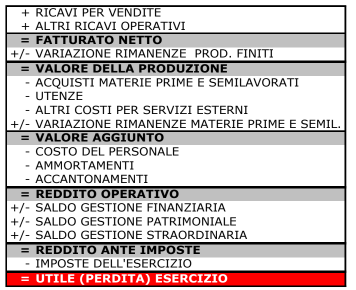
\includegraphics[width=0.5\linewidth]{images/riclassificazione-conto-economico.PNG}
    \caption{Conto economico riclassificato}
    \label{fig:riclassificazione-conto-economico}
\end{figure}

\subsection{Indicatori di bilancio}
Gli \textit{indicatori di bilancio}\index{Organizzazione aziendale!Bilancio!indicatori} o ratio permettono di misurare la performance aziendale da diversi punti di vista:
\begin{enumerate}
    \item \textit{Reddituali:} includono indici di redditività (ROI, ROE) e di economicità (ricavi/costi).
    \item \textit{Finanziari:} riguardano la liquidità e l’indebitamento dell’azienda.
    \item \textit{Patrimoniali:} analizzano la solidità e la solvibilità patrimoniale, ossia la capacità di fronteggiare obbligazioni a lungo termine.
\end{enumerate}

Gli indici di redditività principali sono:
\begin{enumerate}
    \item \textit{ROI (Return on Investment):} misura la redditività del capitale investito rapportando il reddito operativo al capitale investito.
    \begin{equation*}
        ROI = \frac{\textit{REDDITO OPERATIVO}}{\textit{CAPITALE INVESTITO}}
    \end{equation*}
    \item \textit{ROS (Return on Sales):} misura la redditività delle vendite rapportando il reddito operativo ai ricavi.
    \begin{equation*}
        ROS = \frac{\textit{REDDITO OPERATIVO}}{\textit{RICAVI}}
    \end{equation*}
    \item \textit{ROE (Return on Equity):} valuta la redditività del capitale proprio rapportando l’utile ai mezzi propri dell’azienda.
    \begin{equation*}
        ROE = \frac{\textit{UTILE}}{\textit{MEZZI PROPRI}}
    \end{equation*}
\end{enumerate}
Il \textit{ROI} rappresenta il rendimento del capitale investito, calcolato dividendo il reddito operativo per il capitale investito. È un indicatore utile per valutare l’efficacia complessiva della gestione aziendale, mostrando quanto il capitale investito sia stato profittevole. Maggiore è il ROI, migliore sarà la capacità dell’azienda di generare ricchezza dai propri investimenti.

Il \textit{ROE} misura la redditività del capitale proprio, cioè quanto rende agli azionisti il capitale che hanno investito nell’azienda. Si calcola dividendo l’utile netto per il capitale netto (mezzi propri). Un ROE elevato significa che l’azienda sta generando un buon ritorno per gli investitori e rappresenta un indicatore chiave per valutare l’attrattiva dell’azienda per futuri investitori.

Per interpretare correttamente ROI e ROE, è importante confrontarli con il \textit{costo medio ponderato del capitale}\index{Organizzazione aziendale!Bilancio!costo medio ponderato} (WACC) per il ROI e con il \textit{costo del capitale proprio}\index{Organizzazione aziendale!Bilancio!costo del capitale proprio} per il ROE. Un’azienda crea valore quando il rendimento del capitale investito (ROI) è superiore al WACC ($ROI > WACC$). Il WACC rappresenta il costo complessivo del capitale di rischio e di credito, ponderato in base alla proporzione tra mezzi propri e debito. La formula per il WACC è:
\begin{equation*}
    W\text{}ACC=C_{MP}\frac{MP}{(MP+D)}+C_{D}\frac{D}{(MP+D)}
\end{equation*}
Dove $MP$ rappresenta i mezzi propri, $D$ è il debito, $C_{MP}$ è il costo del capitale di rischio, che si può stimare tramite il modello CAPM e $C_D$ è il costo del capitale di debito, ossia il tasso d’interesse sul debito.

Il \textit{Capital Asset Pricing Model} (CAPM) permette di calcolare il costo del capitale di rischio in base alla formula:
\begin{equation*}
    C_{MP}=R_f+\beta(R_m-R_f)
\end{equation*}
Dove $R_f$ è il tasso di rendimento privo di rischio (come quello dei titoli di Stato), $R_m$ è il rendimento atteso del mercato e $\beta$ è il coefficiente che misura il rischio specifico dell’azienda rispetto al mercato. Se $\beta > 1$, l’azienda è più rischiosa del mercato, se $0 < \beta < 1$, l’azienda è meno rischiosa del mercato.